\documentclass[
    parskip=half, 
    twoside=false,
    twocolumn=true,
    fontsize=11pt,
]{scrarticle}
\usepackage{xcolor}
\definecolor{seeblau}{HTML}{00A9E0}
\definecolor{seegrau}{HTML}{9AA0A7}

\definecolor{seeblau1}{HTML}{CCEEF9}
\definecolor{seeblau2}{HTML}{A6E1F4}
\definecolor{seeblau3}{HTML}{59C7EB}
\definecolor{seeblau4}{HTML}{00A9E0}
\definecolor{seeblau5}{HTML}{008ECE}


\usepackage{graphicx}
\usepackage{amsmath}
\usepackage{subcaption}
\usepackage{wrapfig}
\usepackage[english]{babel}
\usepackage{blindtext}
\usepackage{microtype}
\usepackage{siunitx}
\usepackage[utf8]{inputenc}
\usepackage{csquotes}
\usepackage{nicefrac}
\usepackage[T1]{fontenc}
\usepackage{amsfonts}
\usepackage{amssymb}
\usepackage{tikz}

\usepackage{siunitx}

\usepackage{libertinus, libertinust1math}
\usepackage{roboto}

\setkomafont{disposition}{\normalfont\sffamily}


% not recommended with KOMA-script
% make table of contents sans-serif
% \usepackage{tocloft}
% \renewcommand\cftchappagefont{\normalfont}
% \renewcommand\cftchapfont{\normalfont}
% \renewcommand\cftchappresnum{\bfseries}
% \renewcommand\cftchapaftersnum{}
% \renewcommand{\cftchapfont}{\sffamily}
% \renewcommand{\cftsecfont}{\sffamily}
% \renewcommand{\cftsubsecfont}{\sffamily}
% \renewcommand{\cftchappagefont}{\sffamily}
% \renewcommand{\cftsecpagefont}{\sffamily}
% \renewcommand{\cftsubsecpagefont}{\sffamily}

% caption
\usepackage{caption}
\captionsetup{
	% font={sf},
	labelfont={sf, bf, color=seeblau},
	labelsep=quad,
	labelformat=simple,
}

% links
\usepackage{hyperref}
\hypersetup{
	colorlinks=true,
	linkcolor=seeblau,
	citecolor=seeblau,
	urlcolor=seeblau,
	% hidelinks=true
}

% bibliography
\usepackage[
	style=numeric-comp, % comp = compressed 4,5,6,7 -> 4-7
	sorting=none,		% Sort by appearance
	% autocite = superscript,
	% backref=true,
	hyperref=true,
	url=true,
	maxbibnames=100
]{biblatex}
\DefineBibliographyStrings{english}{%
    backrefpage  = {see p.}, % for single page number
    backrefpages = {see pp.} % for multiple page numbers
}

% remove issue
\AtEveryBibitem{%
  \clearfield{number}
}

\usepackage{float}
% \floatplacement{figure}{h}
% \floatplacement{table}{H}

% loosen float placement rules
\renewcommand{\topfraction}{0.8}
\renewcommand{\bottomfraction}{.8}
\renewcommand{\textfraction}{0.1}
\renewcommand{\floatpagefraction}{.9}
% make floats less likely to be placed on a separate page
\setcounter{totalnumber}{9}
\setcounter{topnumber}{9}
\setcounter{bottomnumber}{9}

% decrease space between floats and text
\setlength{\textfloatsep}{0.5cm}
\setlength{\floatsep}{0.5cm}


\usepackage{adjustbox}

\usepackage{datetime}
\newdateformat{dotdate}{
	\twodigit{\THEDAY}.\twodigit{\THEMONTH}.\THEYEAR
}
\newdateformat{monthyeardate}{%
  \monthname[\THEMONTH] \THEYEAR}


% header and footer
\usepackage[
  markcase=noupper
]{scrlayer-scrpage}% activates pagestyle scrheadings automatically
\clearpairofpagestyles
\setkomafont{pageheadfoot}{\normalfont\sffamily}
\setkomafont{pagenumber}{\normalfont\sffamily}
% \chead*{\color{seegrau} Draft \dotdate\today}
\ofoot*{\pagemark}
\ohead*{\rightmark}


\usepackage{ifthen}
\newcommand{\markieren}[4]{
    \ifthenelse{\equal{#1}{}}{}{\adjustbox{padding=3pt, bgcolor=seeblau1, margin=-1pt}{\strut{\sffamily\robotoMedium{#1}}}\\}
    \ifthenelse{\equal{#2}{}}{}{\adjustbox{padding=3pt, bgcolor=seeblau2, margin=-1pt}{\strut{\sffamily\robotoMedium{#2}}}\\}
	\ifthenelse{\equal{#3}{}}{}{\adjustbox{padding=3pt, bgcolor=seeblau3, margin=-1pt}{\strut{\sffamily\robotoMedium{#3}}}\\}
	\ifthenelse{\equal{#4}{}}{}{\adjustbox{padding=3pt, bgcolor=seeblau4, margin=-1pt}{\strut{\sffamily\robotoMedium{#4}}}}
}

\addbibresource{literature.bib}

\begin{document}

\title{title}
\subtitle{subtitle}
\author{Aurel Müller-Schoenau, Leon Oleschko}
\date{\dotdate\today}


% make a custom title page
\begin{titlepage}
    \sffamily
    \vspace*{3cm}
    {
        \fontsize{32}{32}
        \markieren{}{}{Evanescent light scattering}{Optical Tweezers}
    }
    \vspace{.25cm}\\
    {
        \Large
        Aurel Müller-Schoenau, Leon Oleschko\\
        Supervised by Krishna Kumar, Karthika
        \vspace{.05cm}\\
        13.11.2024
        \vspace{.25cm}\\
        \normalsize
        Physikalisches Fortgeschrittenenpraktikum 2\\
        Universität Konstanz
    }
    \vfill
    {
        \normalfont\normalsize
        Abstract auf Englisch (10-15 Zeilen)
        \blindtext[2]
    }
    \vfill
    \begin{flushright}
        Available at \url{www.github.com/leoole100/fp2}.
    \end{flushright}
\end{titlepage}

\section{Introduction}

\subsection{Physical Principles}
kompakten Zusammenstellung der physikalischen Grundlagen

Mean square deviation and velocity autocorrelation:
\url{https://de.wikipedia.org/wiki/Mittlere_quadratische_Verschiebung#Verbindung_zur_Geschwindigkeitsautokorrelation}
\begin{align}
    &&\left<v(t)\cdot v(t+\tau)\right> &= - \frac{d}{d\tau} \frac{\left<r^2(\tau)\right>}{6\tau}\\
    \Rightarrow&&\left<r^2(\tau)\right> &= 6 \int_0^\tau (\tau - s) \left<v(0) \cdot v(s)\right> ds
\end{align}

The maxwell boltzmann relations (from script) are given by
\begin{align}
    P(x) &\propto \exp\left(- \frac{V(x)}{k_B T}\right)\\
    V(x) &\propto - \frac{\log{P(x)}}{k_B T}
\end{align}


\section{Methods}
Mit einer Skizze des Versuchsaufbaus

\section{Procedure}

\section{Results}
All recorded data and the analysis is available at \url{www.github.com/leoole100/fp2}.

\pagebreak
\subsection{Transmission Light Microscopy}
\begin{figure}
    \centering
    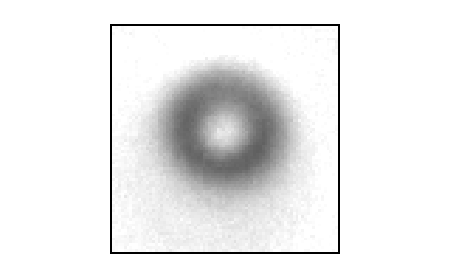
\includegraphics{figures/01_01_1_particle.pdf}
    \caption{Transmission light microscopy of a observed particle. The radius of the particle is \SI{14(2)}{px}, equivalent to \SI{1.86(27)}{\micro m}.}
    \label{fig:01particle}
\end{figure}
In the first section of the experiment, the particles were observed using a transmission light microscope setup.
For this images with a resolution of $600\times 800$\si{px} were recorded with a frequency of \SI{10}{Hz} for \SI{10}{min}.
The images were normalized with a black (illumination off) and white (illumination on, particle not in frame) reference image, to remove the influence of dust in the imaging elements.
The particle that was used for this experiment is shown in \autoref{fig:01particle}, after the normalization.

CONVERSION PX TO MICROMETER

\begin{figure*}
    \centering
    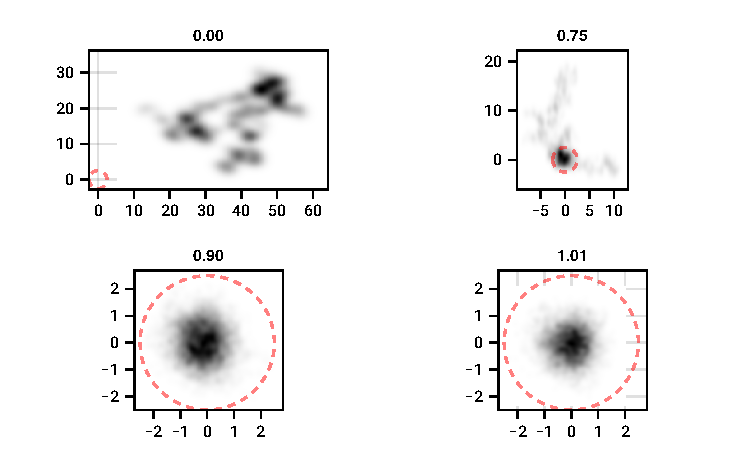
\includegraphics{figures/01_03_1_bivariate.pdf}
    \caption{Density of recorded particle positions, grouped by optical trap stiffness. The red circle indicates the approximate radius of the optical trap \SI{2.5}{\micro m}.}
    \label{fig:01bivariate}
\end{figure*}
To determine the trajectory of the particle, a effective center of mass was calculated for each frame:
\begin{equation}
    \vec{r}(t) = \iint \vec{r} \cdot \left(1-I(\vec{r}, t)\right)^2 d\vec{r}    
\end{equation}
The density of the resulting trajectory is shown in \autoref{fig:01bivariate} for different optical trap stiffnesses.
The approximate radius of the optical trap of \SI{2.5}{\micro m} is drawn as a red circle.
For the trap stiffness of \SI{0}{}, the particle is free to wander around, for the higher stiffnesses like \SI{1.01}{} the particle is mostly confined to the trap.\\
For a weak trap like \SI{0.75}{} the particle is still mostly confined to the trap, but can escape the linear trap region and randomly wander around. 
This happened multiple times during the shown measurement.

\begin{figure}
    \centering
    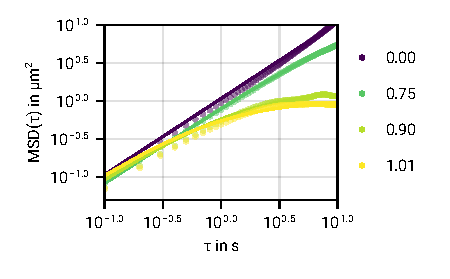
\includegraphics{figures/01_02_2_msd.pdf}
    \caption{Mean Square Displacement for different optical trap stiffnesses, fit: \autoref{eq:01_mdl_msd}}
    \label{fig:01msd}
\end{figure}
\subsection*{Mean Square Displacement}
A method to describe the trajectory of a random walk is the mean square displacement (MSD) \cite{wiki:msd}.
This is defined as the average of the squared distance of the particle from the starting point:
\begin{equation}
    \text{MSD}(t) = \left<\Delta r^2(t)\right> = \frac{1}{N} \sum_i^N \left(x_i(t) - x_i(0) \right)^2 
\end{equation}
Here a different implementation using the autocorrelation of the velocity was used, to achieve a more stable result.
This was implemented by \cite{jl:msd}.
The resulting MSD for different optical trap stiffnesses is shown in \autoref{fig:01msd}.

This can be described as 

Model for the MSD with $k=\alpha P \cdot\nicefrac{k_B T}{\text{MSD}(\infty)}$ with the optical tweezer power $P$ in arbitrary units:
\begin{align}
    \frac{1}{\text{MSD}(\tau, k)}
    &= \frac{1}{D_0 \tau} + \frac{1}{\text{MSD}(\infty)}\\
    &= \frac{1}{D_0 \tau} + \frac{1}{(k_B T \cdot P)_i}
    \label{eq:01_mdl_msd} 
\end{align}
For the $i$-th measurement.


\begin{figure}
    \centering
    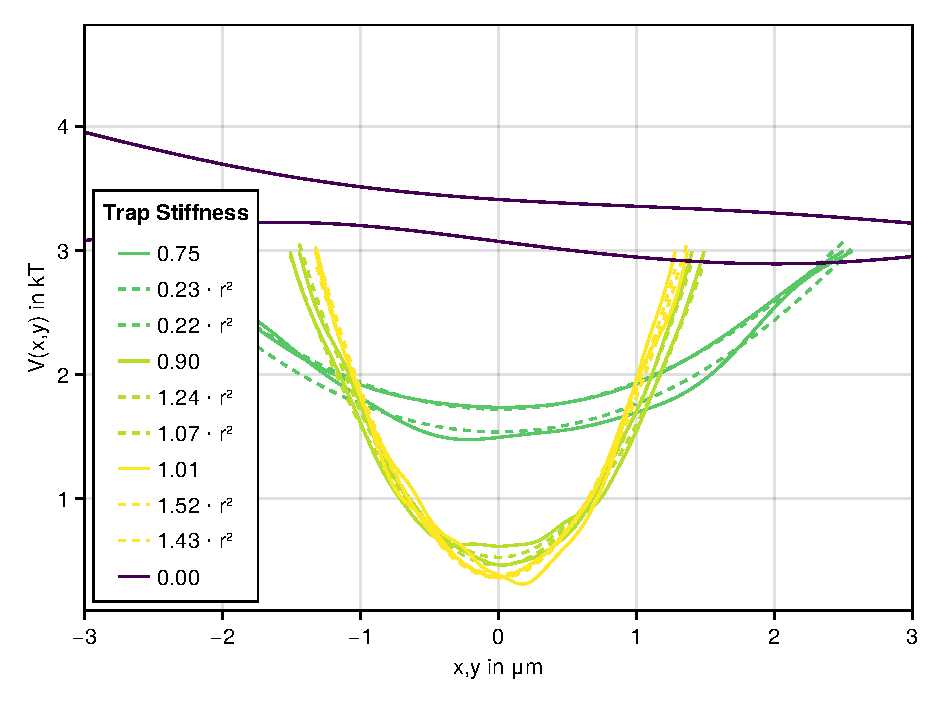
\includegraphics{figures/01_03_3_axis.pdf}
    \caption{Grouped by axis, relative to mean.}
\end{figure}

\begin{figure}
    \centering
    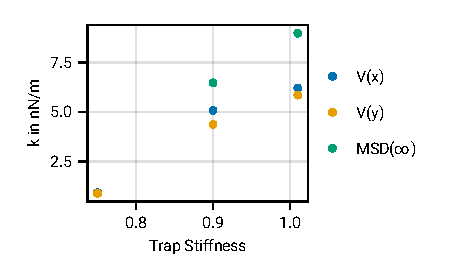
\includegraphics{figures/01_03_4_spring_constants.pdf}
    \caption{Differently measured spring constants.}
\end{figure}

\clearpage
\subsection{Total Internal Reflection Microscopy}
\begin{align}
    P(\Delta z) &= N(0, \sigma^2) = N\left(0, \frac{\Delta T}{\left<T_s\right>} \sigma_s^2\right)\\
    \Delta I &= - I_0 \beta \exp\left(-\frac{z}{\beta}\right) \Delta z \\
    P(\Delta I) &= P(\Delta z) \left|\frac{d \Delta z}{d \Delta I}\right|\\
    &= N(0, \sigma^2) \;\frac{1}{I_0\beta} \exp\left(\frac{z}{\beta}\right)
\end{align}


\clearpage
\section{Discussion}
\blindtext

\addcontentsline{toc}{section}{Literature}
\nocite{*}
\printbibliography

\end{document}